\chapter{Eine kurze Einführung in die Programmierumgebung mBlock}

Das Programm \href{http://www.mblock.cc/}{mBlock} ist eine graphische Programmierumgebung, die auf Scratch beruht und es sehr einfach macht, erste Programmiererfahrungen zu sammeln. Abbildung \ref{abb:mblock-uebersicht} zeigt eine grobe Übersicht über die einzelnen Elemente des Programms, jedoch lernt man sie am besten kennen, indem man einfach drauf loslegt und ausprobiert, was sich damit anstellen lässt.


\begin{figure}[H]
	\begin{adjustwidth*}{-1.5cm}{-1.5cm}
	\centering
	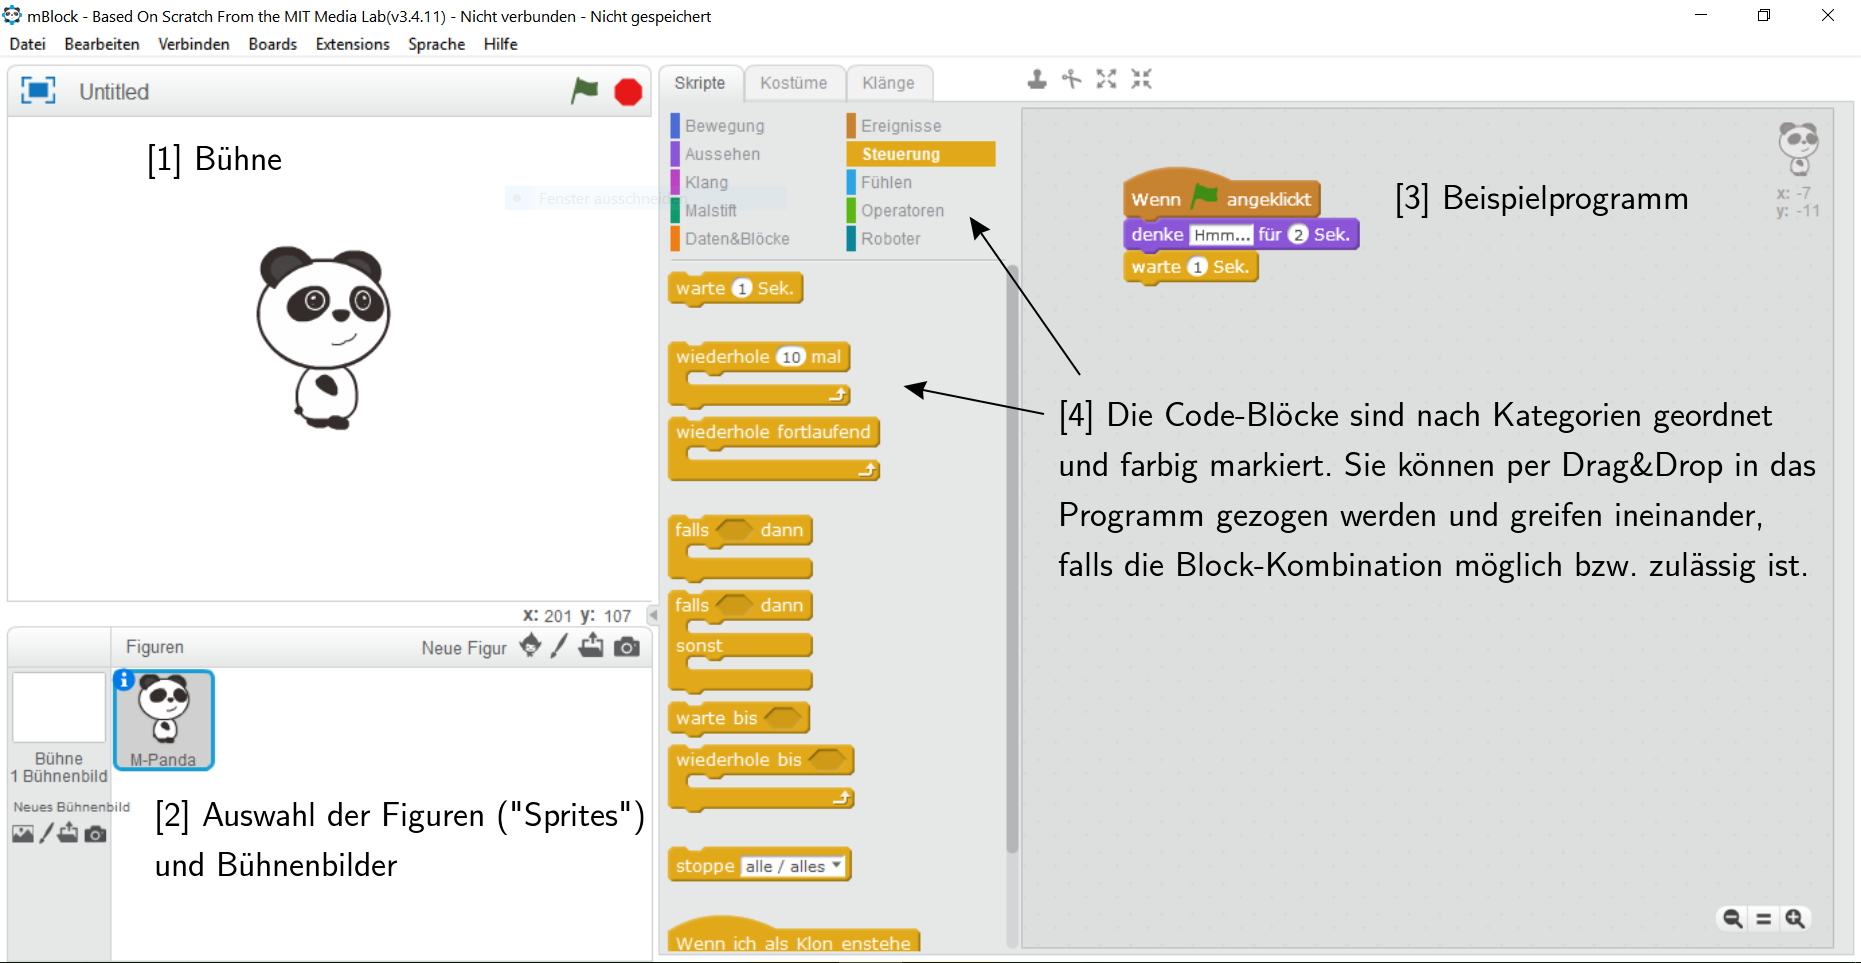
\includegraphics[width=1.2\textwidth]{pics/mblock-uebersicht.PNG}
	\caption{Übersicht über die Programmierumgebung \emph{mBlock}.}
	\label{abb:mblock-uebersicht}
	\end{adjustwidth*}
\end{figure}

	
Für die ersten Programmiererfahrungen machen wir noch nichts mit dem Arduino, sondern kümmern uns nur um die in mBlock eingebaute Bühne.

\marginpar{%
	\textattachfile[description={Folie zu Kap. \thechapter, Auftrag Pandalauf}]{./Auftraege/kap1-auftrag-pandalauf.pdf}{%
	\footnotesize%
	\folie Folie%
	}%
	%\href{run:./Auftraege/kap1-auftrag-pandalauf.pdf}{Folie}\\%
	\footnotesize
	\\öffnen%
}
\begin{ziel}
	\textbf{Ziel:} Der Panda soll auf der Bühne folgendes machen, nachdem auf die grüne Fahne ($\rightarrow$ Ereignisse) geklickt wurde:
	\begin{itemize}[itemsep=0ex]
		\item Der Panda läuft von links nach rechts. ($\rightarrow$ Bewegung)
		\item Der Panda sagt für 1 Sekunde \enquote{Hallo!}. ($\rightarrow$ Aussehen)
		\item Der Panda läuft von rechts nach links.
		\item Der Panda wartet eine Sekunde (und macht dabei nichts).
		\item Der ganze Vorgang wiederholt sich fortlaufend.
	\end{itemize}
\end{ziel}

\emph{Für Schnelle und Kreative:} Erweitere dein Programm, indem du eine andere Bühne oder ein anderes Kostüm auswählst. Spiele mit den Befehlen herum, um dein Programm individuell anzupassen.

\begin{zsfg}{{Programm, Befehl und Argument}}
	\begin{wrapfigure}{r}{0.3\textwidth}
	   \centering
	   
\includegraphics[width=0.3\textwidth]{pics/Befehl-Bsp.png}
	   \caption{Befehl mit Textargument und Zahlargument.}
	   \label{abb:befehlbsp}
	\end{wrapfigure}
	Ein Programm besteht aus einer Folge von Anweisungen oder Befehlen. Man spricht auch von Algorithmen: Ein Algorithmus ist eine eindeutige Handlungsvorschrift zur Lösung eines Problems, die aus endlich vielen Anweisungen besteht (s. \href{https://de.wikipedia.org/wiki/Algorithmus}{Wikipedia}).
	
	Ein Befehl \emph{kann} ein oder mehrere \emph{Argumente} haben, die wiederum einen unterschiedlichen Typ haben können (z.\,B. Text oder (ganze) Zahl).
\end{zsfg}

\begin{aufgabe}
	\textit{Gehübungen}\smallbreak
	Beschreibe jeweils, was der Panda macht, wenn das abgebildete Programm läuft. Streiche, wenn möglich, alle Befehle, die man nicht benötigt.
\end{aufgabe}
\begin{figure}[H]
	\centering
	\subfloat[]{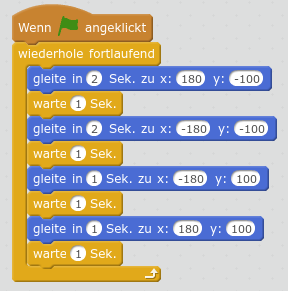
\includegraphics[width=0.37\textwidth]{pics/panda-rechtecklauf.png}}
	\hspace{0.5cm}
	\subfloat[]{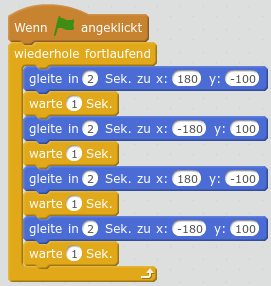
\includegraphics[width=0.35\textwidth]{pics/panda-diagonalenlauf.png}}
	\label{abb:uebungsbsp_befehle}
\end{figure}